\section*{Синтез стабилизирующих регуляторов}

\subsection*{Управляемая система 1}

Рассмотрим систему:
\begin{align}
\dot{x}_1 &= -x_1 + 2x_1^3 + x_2 + \sin u_1 \\
\dot{x}_2 &= -x_1 - x_2 + 3\sin u_2
\end{align}

\subsubsection*{Выбор целевой точки и линеаризация по отклонениям}

Стабилизируем систему к точке вида $(1,x^*)$, где $x^*\in[-2,0]$ (это условие необходимо и достаточно для существования стационарных входов, см. ниже) и $x^*\neq -1$.
Из условий равновесия $f(1,x^*,u_{ss})=0$ получаем
\[
\sin u_{1,ss} = -(1+x^*),\qquad \sin u_{2,ss} = \frac{1+x^*}{3}.
\]
Для конкретики берём $x^*=-1.5$, тогда $u_{1,ss}=\arcsin(0.5)=\pi/6\approx0.524$, $u_{2,ss}=\arcsin(-0.5)= -\pi/6\approx-0.167$.
Линеаризуем систему по отклонениям $\tilde x = x - x^*$ и $v = u - u_{ss}$.

Матрицы Якоби в точке $(x^*,u_{ss})$ имеют вид:
\begin{align*}
A &= \left.\frac{\partial f}{\partial x}\right|_{(x^*,u_{ss})} =
\begin{pmatrix}
-1 + 6x_1^2 & 1 \\
-1 & -1
\end{pmatrix}_{x^*} =
\begin{pmatrix}
5 & 1 \\
-1 & -1
\end{pmatrix}, \\
B &= \left.\frac{\partial f}{\partial u}\right|_{(x^*,u_{ss})} =
\begin{pmatrix}
\cos u_{1,ss} & 0 \\
0 & 3\cos u_{2,ss}
\end{pmatrix} =
\begin{pmatrix}
\cos(\pi/6) & 0 \\
0 & 3\cos(-\pi/6)
\end{pmatrix} =
\begin{pmatrix}
0.8660 & 0 \\
0 & 2.9580
\end{pmatrix}.
\end{align*}

\subsubsection*{Синтез LQR}

Выберем $Q = 10I$, $R = I$ и решим алгебраическое уравнение Риккати
\[ A^T P + PA - PBR^{-1}B^T P + Q = 0,\quad K = R^{-1}B^T P. \]
Получаем матрицу обратной связи (численно)
\[
K = \begin{pmatrix}
11.7429 & 0.7194 \\
2.4573 & 3.0173
\end{pmatrix}.
\]
Спектр замкнутой линейной системы:
\[ \sigma(A-BK) = \{-5.9547,\;-9.1401\}. \]
Цель $(1,-1.5)$ локально экспоненциально устойчива; моделирование подтверждает сходимость траекторий к окрестности этой точки.

\subsection*{Управляемая система 2}

Рассмотрим систему:
\begin{align}
\dot{x}_1 &= x_2 + x_1 x_2 + u \\
\dot{x}_2 &= -x_2 + x_2^2 - x_1^3 + \sin u
\end{align}

\subsubsection*{Поиск точек равновесия}

При $u = 0$ система принимает вид:
\begin{align}
\dot{x}_1 &= x_2 + x_1 x_2 \\
\dot{x}_2 &= -x_2 + x_2^2 - x_1^3
\end{align}

Точки равновесия находятся из решения:
\begin{align}
x_2(1 + x_1) &= 0 \\
- x_2 + x_2^2 - x_1^3 &= 0
\end{align}

\textbf{Случай 1:} $x_2 = 0$. Из второго уравнения: $-x_1^3 = 0 \Rightarrow x_1 = 0$

\textbf{Случай 2:} $x_1 = -1$. Из второго уравнения: $-x_2 + x_2^2 - (-1)^3 = 0 \Rightarrow x_2^2 - x_2 + 1 = 0$.
Дискриминант: $D = 1 - 4 = -3 < 0$ --- нет действительных решений.

\textbf{Точка равновесия:} $(0, 0)$

\subsubsection*{Выбор точки равновесия и линеаризация}

Выберем точку равновесия $(x_1^*,x_2^*) = (0,0)$ и установим стационарный вход $u_{ss} = 0$.

Матрицы линейной модели:
\[
A = \begin{pmatrix} 0 & 1 \\ 0 & -1 \end{pmatrix},\qquad
B = \begin{pmatrix} 1 \\ 2 \end{pmatrix}.
\]
Для $Q=10I$, $R=1$ получаем
\[
K = \begin{pmatrix} 3.1623 & 2.1014 \end{pmatrix},\qquad
\sigma(A-BK) = \{-1.3529,\;-7.0121\}.
\]

\subsection*{Численное моделирование}

Результаты численного моделирования показывают эффективность синтезированных LQR регуляторов: для системы 1 траектории сходятся к точке $(1,-1.5)$, для системы 2 --- к $(0,0)$.

\begin{figure}[H]
\centering
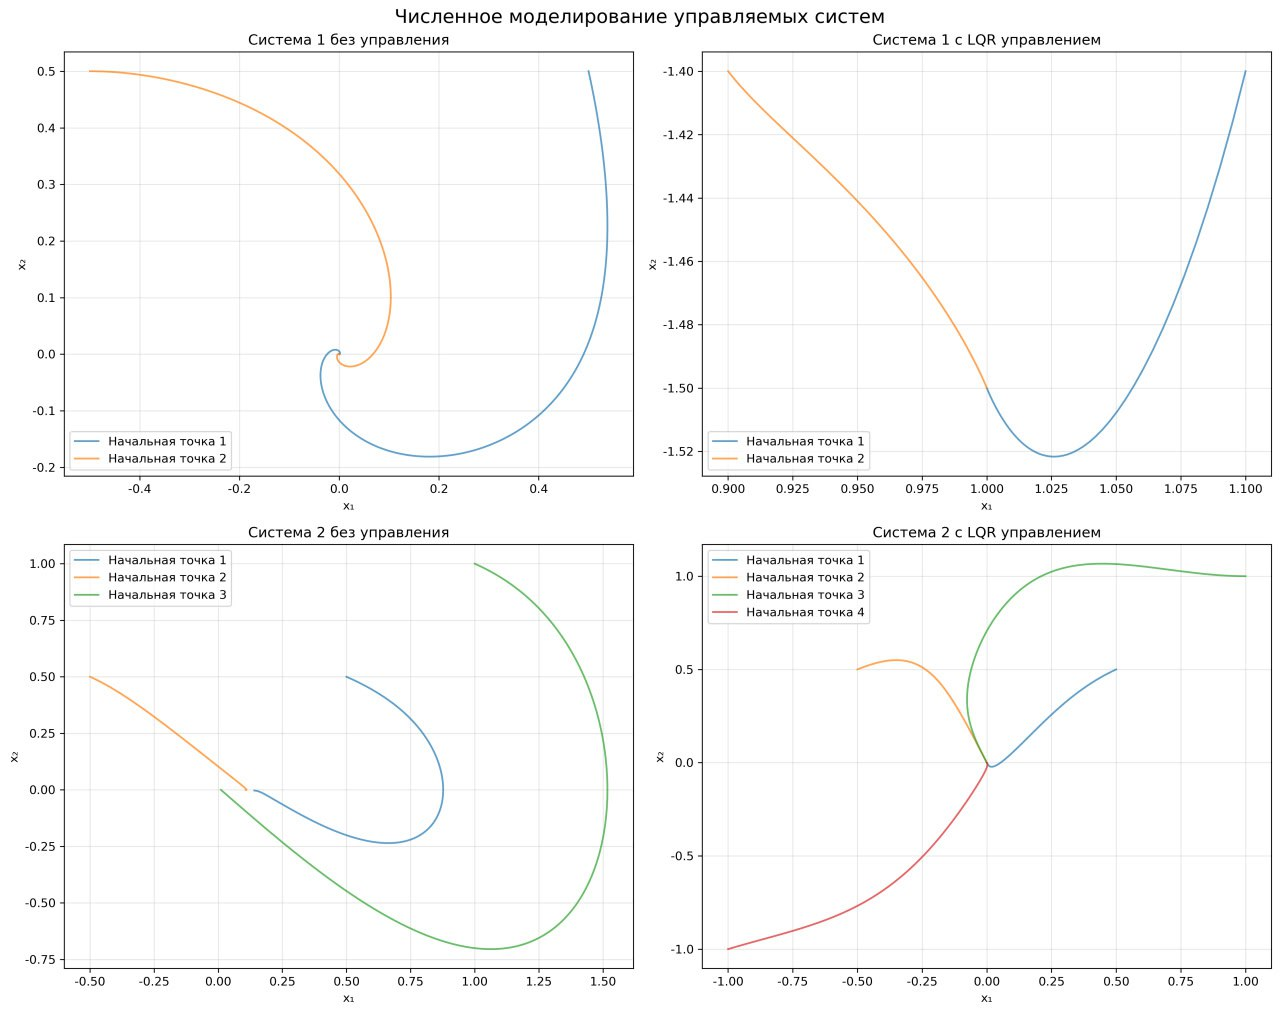
\includegraphics[width=0.8\textwidth]{controlled_systems/controller_simulation.png}
\caption{Результаты численного моделирования управляемых систем}
\label{fig:controller_sim}
\end{figure}
